\subsubsection{UC12 - Esecuzione funzione}
\begin{figure}[h]
	\centering
	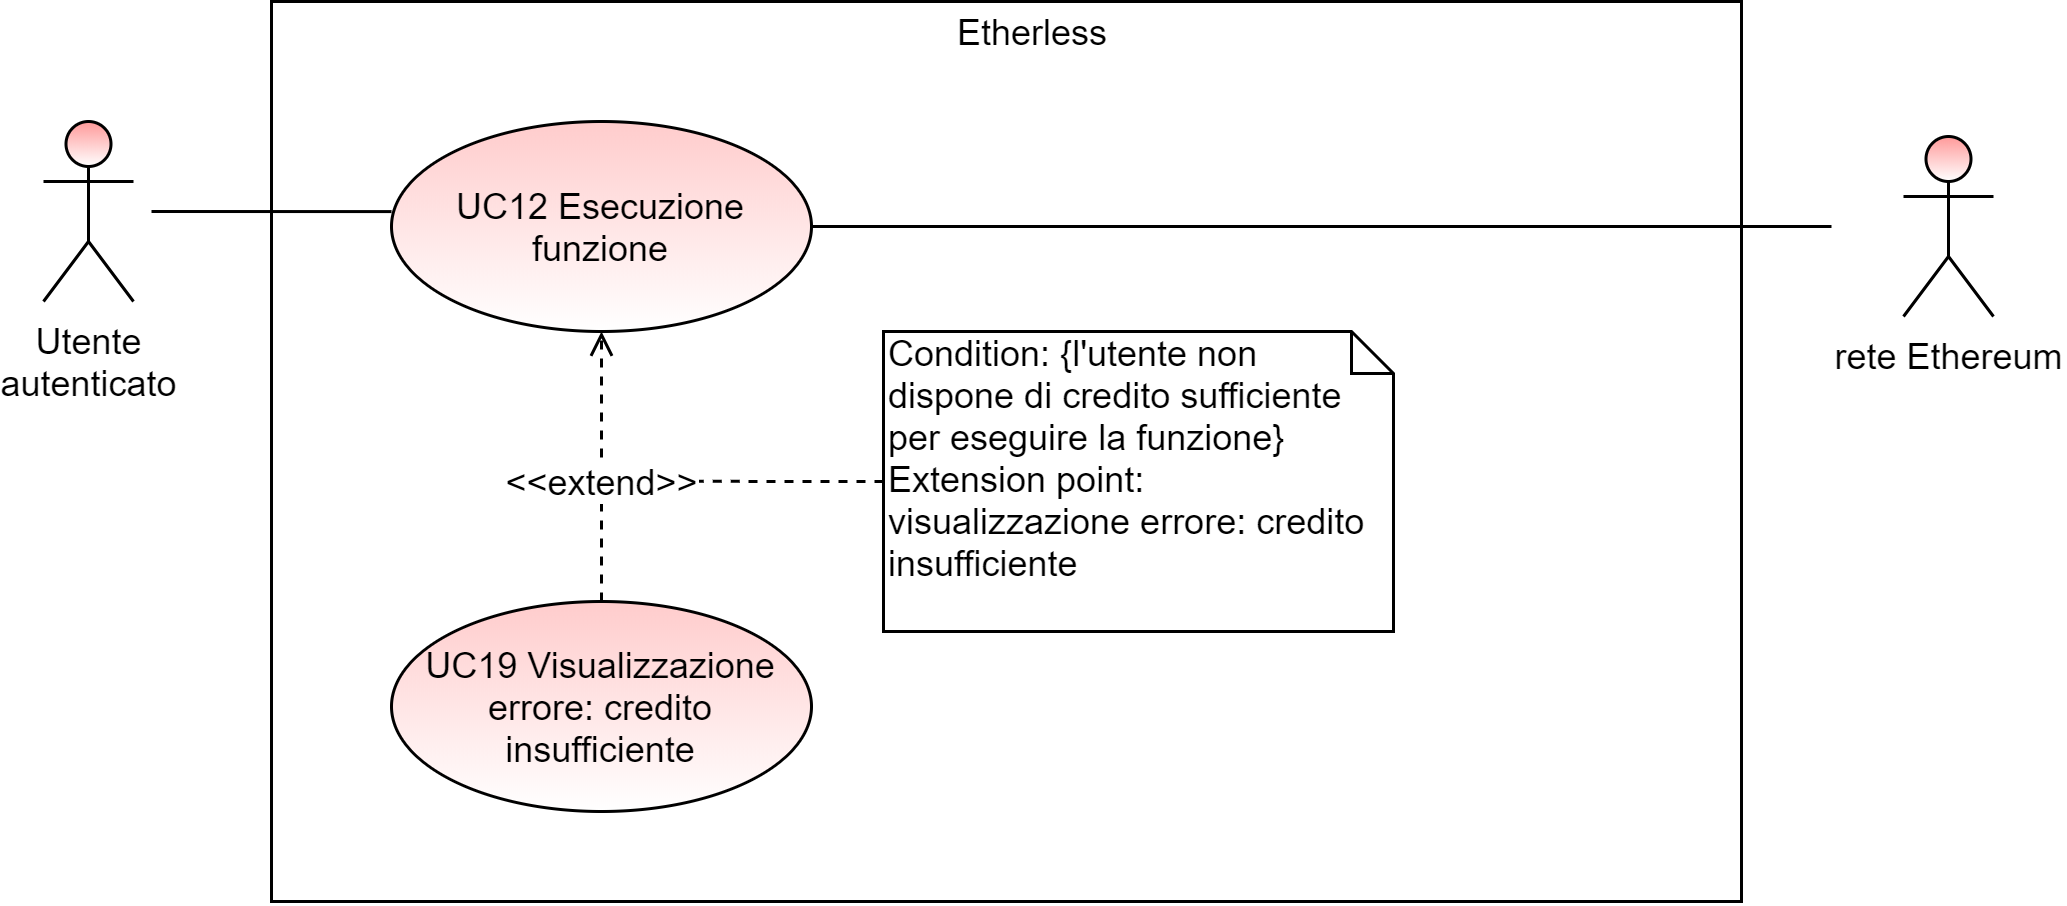
\includegraphics[scale=\ucs]{./res/img/UC12G.png}
	\caption {UC12 - Esecuzione funzione: schema generale}
\end{figure}
\begin{figure}[h]
	\centering
	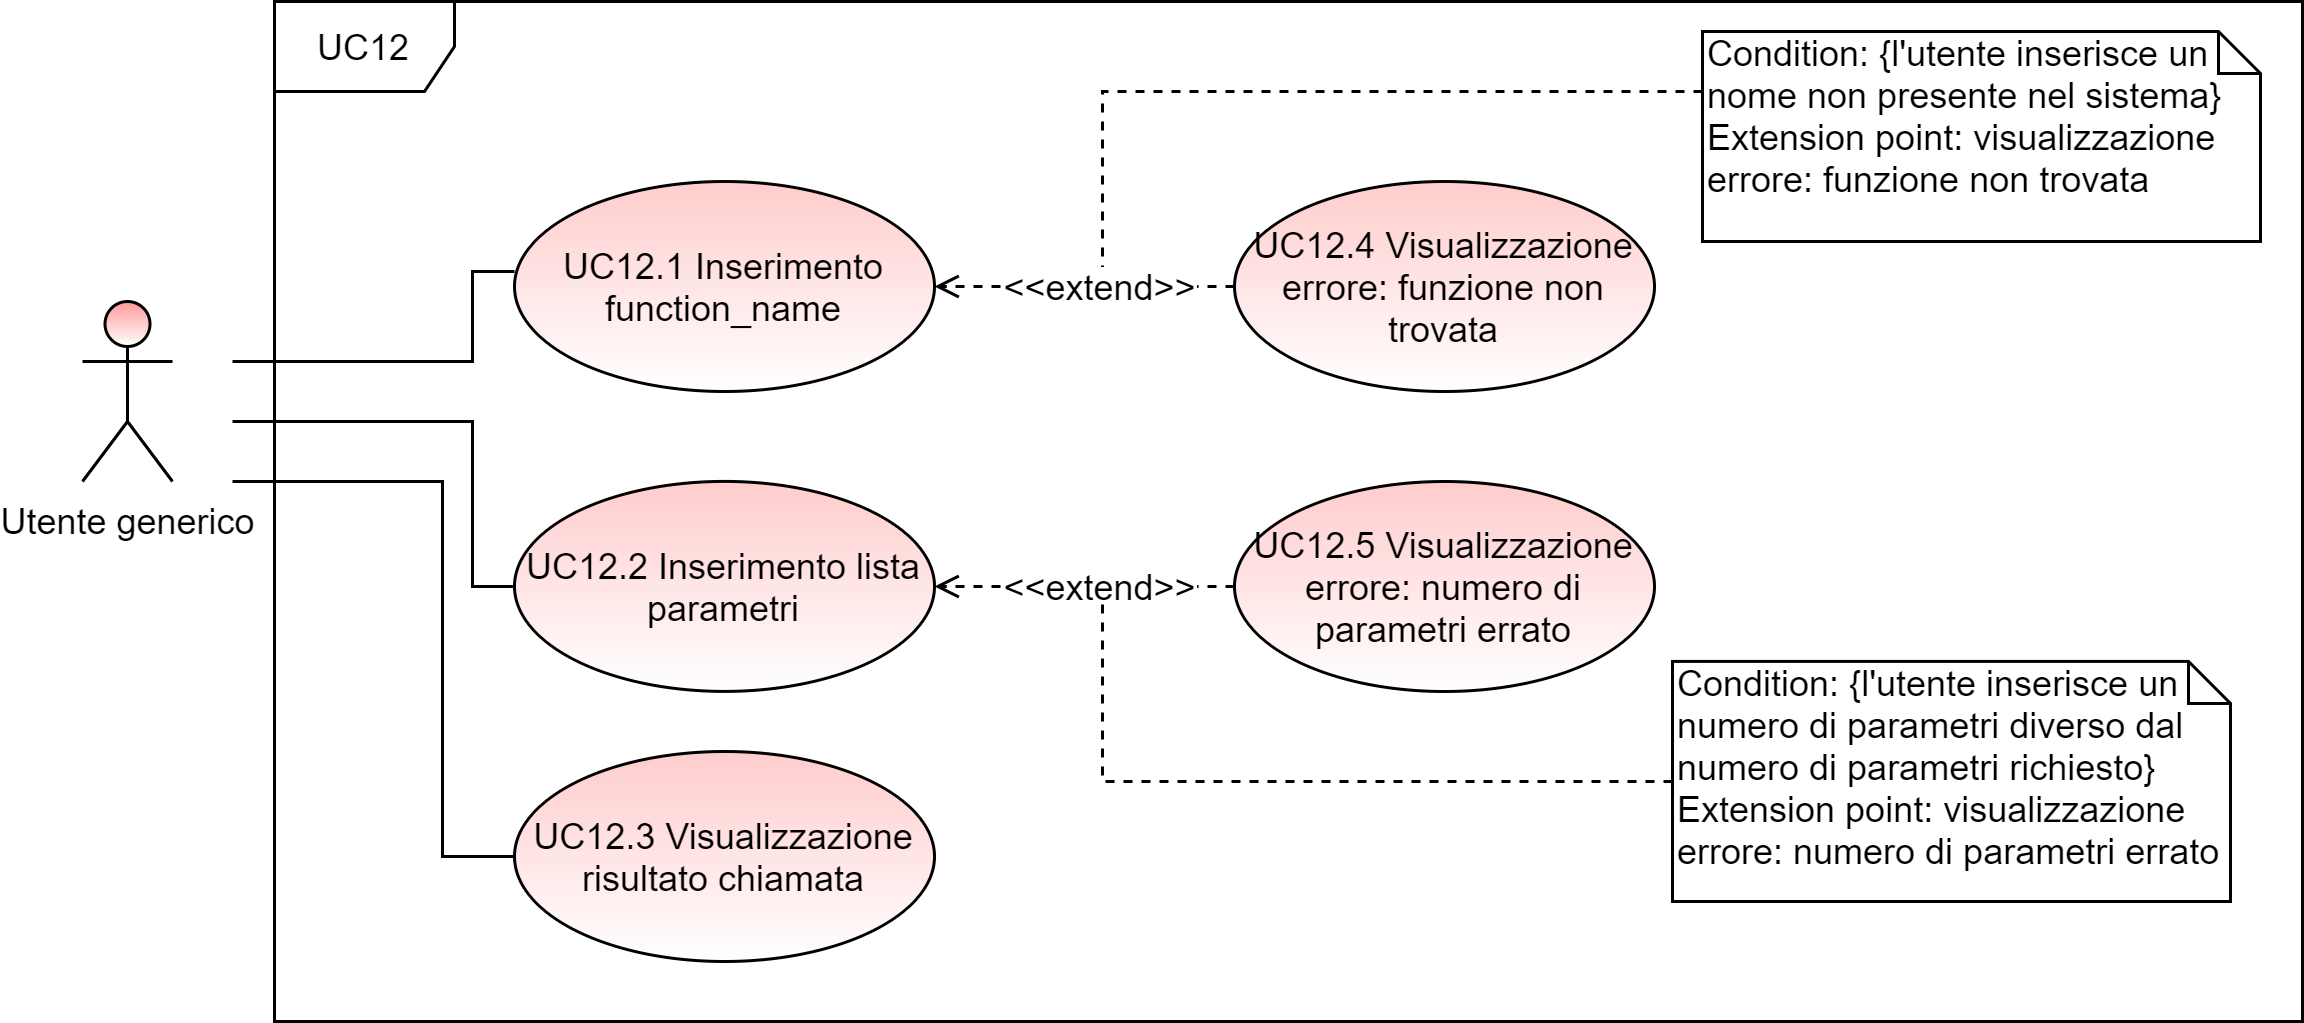
\includegraphics[scale=\ucs]{./res/img/UC12.png}
	\caption {UC12 - Esecuzione funzione}
\end{figure}
\begin{itemize}
	\item \textbf{Attori primari:} \ua{};
	\item \textbf{Attori secondari:} \re{};
	\item \textbf{Descrizione:} l’utente richiede l’esecuzione di una delle funzioni presenti nel sistema eseguendo il comando \prun{}. Il sistema stampa a video il risultato di tale chiamata; 
	\item \textbf{Scenario principale:} 
	\begin{itemize}
		\item l'utente inserisce correttamente ed esegue il comando \prun{}; 
		\item viene visualizzato il risultato dell’esecuzione. 
	\end{itemize}
	\item \textbf{Estensioni:} 
	\begin{itemize}
		\item \textbf{UC19:} l’utente non dispone di credito sufficiente per portare a termine l’esecuzione della funzione, di conseguenza viene visualizzato un messaggio di errore.
	\end{itemize}
	\item \textbf{Precondizione:} l’utente si è autenticato all’interno della piattaforma e vuole eseguire una delle funzioni disponibili;
	\item \textbf{Postcondizione:} la CLI\ped{\textit{G}} riporta il risultato dell’esecuzione della funzione. 
\end{itemize}